\documentclass[sans]{beamer}

\mode<presentation>
{
	% \usetheme{CambridgeUS}
	% \usetheme{Hannover}
	\usetheme{Singapore}
	\usecolortheme{default}
}

\usepackage{cmap}
\usepackage{listings}
\usepackage{lmodern}
\usepackage{color}
\usepackage{minted}
\usepackage{graphicx}
\usepackage{tikz}
\usetikzlibrary{arrows}
\usepackage{wrapfig}
\usepackage{bussproofs}
\usepackage{stmaryrd}
\usepackage{wasysym}

\usepackage[labelformat=empty]{caption}
\usepackage{fontspec}
% \usepackage{polyglossia}
% \setdefaultlanguage{russian}

% \setmainfont[Ligatures=TeX]{DejaVu Serif}
% \setsansfont[Ligatures=TeX]{DejaVu Sans}
% \setmonofont{DejaVu Sans Mono}

\definecolor{myGray}{RGB}{80,80,80}
\EnableBpAbbreviations

\begin{document}

\title
[Concurrency Control]
{Concurrency Control: Methods, Performance, and Analysis}

\subtitle{Based on Alexander Thomasian paper}

\author
[Podkopaev]{Anton Podkopaev, podkoav239@gmail.com}
\institute{SPbSU}
\date [21-11-14]{21 november 2014}

\begin{frame}[plain]
	\titlepage
\end{frame}

\section{Introduction}

\begin{frame}{Main Line}
  \begin{itemize}
    \item Comparison of locking methods

    \item Sources of performance degradation with standard locking:
      \begin{itemize}
        \item Blocking
        \item Deadlock
      \end{itemize}

    \item Restart-oriented locking methods
    \item Waith-depth-limited (WDL) methods

    \item Restart waiting
  \end{itemize}
\end{frame}

\begin{frame}{Notions}
  \begin{itemize}
    \item Work only with correctness criterion as serializability
    \begin{itemize}
      \item It isn't suitable for systems like trading bids
    \end{itemize}
    
    \item Strict 2PL
    \begin{itemize}
      \item Locks to be released only when the txn is
            commited or aborted
      \item To solve cascading aborts
    \end{itemize}

    \item Work only with centralized high-performance systems
  \end{itemize}
\end{frame}

\begin{frame}{Method Sets}
  \begin{itemize}
    \item Restart-oriented locking
    \begin{itemize}
      \item Wait-depth-limited (WDL)
    \end{itemize}

    \item Two-phase processing methods
    \begin{itemize}
      \item Txn re-execution may not require disk I/O
            in case of big buffer
    \end{itemize}
    \item Optimistic CC (OCC)
    \begin{itemize}
      \item Viable for two-phase processing
    \end{itemize}
    \item Time-stamp ordering (TSO)
    \begin{itemize}
      \item For distributed databases
    \end{itemize}
  \end{itemize}
\end{frame}

\section{Model}

\begin{frame}{Hardware and Data Resource Contention}
  \begin{itemize}
    \item Hardware contention
    \begin{itemize}
      \item The primary effect on performance
    \end{itemize}
    \item Data contention
    \begin{itemize}
      \item The secondary effect
    \end{itemize}
  \end{itemize}
\end{frame}

\begin{frame}{Transaction Structure}
  \begin{itemize}
    \item Considering
      \begin{itemize}
        \item Only flat txns
        \item Mostly short update transactions
      \end{itemize}

    \vfill

    \item A txn accessing $k$ objects consists of
      $k + 1$ steps ($C_k$ --- class of txn)
    \item Each step involves CPU processing and disk accesses
    \item After last step --- \emph{commit}
    \begin{itemize}
      \item Locks held by txn are released
    \end{itemize}

  \end{itemize}
\end{frame}

\begin{frame}{Transaction Arrival Process}
  \begin{itemize}
    \item $S$ --- a number of sources
    \item $Z$ --- a think time
    \item $M$ --- a number of txn already at the system
    \vfill
    \item $\Lambda(M) = (S - M)/Z$ --- the arrival rate

    \vfill
    \item \emph{The user isn't involved after the txn is submitted}
  \end{itemize}
\end{frame}

\begin{frame}{System Categories}
  \begin{itemize}
    \item \emph{Open} system --- sufficently large $S$
    \begin{itemize}
      \item The \emph{mean response time characteristic} can be used for the
            performance comparison of CC methods
    \end{itemize}
    \item \emph{Closed} system --- $S = M$ and $Z = 0$
    \begin{itemize}
      \item Can be used to estimate the peak performance of CC methods
      \item Throughput $T(M), M \geq 1$ 
    \end{itemize}
  \end{itemize}
\end{frame}

\begin{frame}{Frequency-based Model}
  \begin{itemize}
    \item The fraction $f_k$  of txns in $C_k$
    \vfill

    \item Open systems
    \begin{itemize}
      \item $\Sigma^K_{k = 1} f_k = 1, f_k \geq 0$
      \item The arrival rate $\lambda_k = \lambda f_k$
      \item $R_k$ --- the mean response time of txns in $C_k$
      \item The mean number of txns in $C_k$ is $M_k = \lambda_kR_k$
    \end{itemize}
    \vfill
    \item Closed systems
    \begin{itemize}
      \item $M_k$ --- transaction concurrency in $C_k$
      \item Immediately relacing of txn in $C_k$ with probability $f_k$
      \item Throughput in $C_k$ --- $T_k(M) = f_k T(M)$
    \end{itemize}
  \end{itemize}
\end{frame}

\begin{frame}{Database Access Model}
  \begin{itemize}
    \item The \emph{granule} --- the unit of data at which CC is applied to the DB
    \begin{itemize}
      \item Page-level \emph{or} Record-level lock
    \end{itemize}
    \item $D$ --- a number of objects in the DB
    \item DB objects are accessed with probabilities
    \begin{itemize}
      \item In most studies --- uniform probability
      \item Another way --- the hot-spot model, $b$ -- $c$ rule 
    \end{itemize}
  \end{itemize}
\end{frame}

\begin{frame}{Computer System Model (1)}
  \begin{itemize}
    \item A queueing network model (QNM)
    \item The CPU processing time --- txn path-length and CPU speed
    \item The disk processing time --- disk access time and the number of disk I/Os
    \item The infinite-resource model
    \begin{itemize}
      \item Useful in comparing the performance limits of CC methods
      \item Each txn has its own virtual CPU and execution time is independent of concurrent txns
    \end{itemize}
    \item The finite-resource model
    \begin{itemize}
      \item Important in case of comparision restart-oriented CC methods with blocking-oriented ones
    \end{itemize}
  \end{itemize}
\end{frame}

\begin{frame}{Computer System Model (2)}
  \begin{columns}

  \begin{column}{.5\linewidth}
    \begin{itemize}
      \item $p_0$ --- a probability of success at current tick
      \item $P_k = p_0 (1 - p_0)^{k - 1} \approx 1/p_0$
      \item $p_n$ --- a probability of access $n$th disk
      \item The number of $n$th disk visits --- $p_n/p_0$
    \end{itemize}
  \end{column}
  \begin{column}{.6\linewidth}
    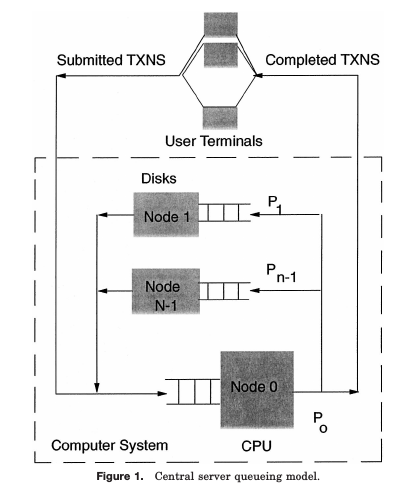
\includegraphics[width = \linewidth]{images/qnmScheme.png}
  \end{column}

  \end{columns}
\end{frame}


\begin{frame}{Computer System Model (3)}
  \begin{itemize}
    \item Product form QNM
    \item Hierarchical solution method
  \end{itemize}
\end{frame}

\begin{frame}{Performance Degradation due to CC Methods}
  \begin{itemize}
    \item No (or negligible) wasted processing
      \begin{itemize}
        \item $T(M) \approx t(M_a)$
      \end{itemize}
    \item Restarts but no blocking
      \begin{itemize}
        \item The system efficiency --- $T(M) / t(M)$
      \end{itemize}
    \item Blocking and restarts
      \begin{itemize}
        \item The system efficiency --- $T(M_a) / t(M_a)$
      \end{itemize}
  \end{itemize}
\end{frame}

\begin{frame}{Separation of Hardware and Data-resource Contention}
  \begin{itemize}
    \item Desirable property --- allows the system-throughput 
      characteristic (STC) to be computed only once
    \item Possible in case of insignificant or independent of
      the level of lock data contention overhead
  \end{itemize}
\end{frame}

\section{Standard Locking}

\begin{frame}{Standard Locking Notions}
  \begin{itemize}
    \item Dynamic locking (DL)
    \item Static locking (SL)
    \item Strict 2PL
      \begin{itemize}
        \item Locks are released at txn completion time 
      \end{itemize}
    \item General Waiting (GW) method
  \end{itemize}
\end{frame}

\begin{frame}{Deadlock resolve techiques (1)}
  \begin{itemize}
    \item The victim selection policies
    \begin{enumerate}
      \item Current blocker
      \item Random blocker
      \item The txn with minimum number of locks
      \item The youngest txn
      \item The txn with minimum amount of work 
    \end{enumerate}
    \item Deadlock resolution policy has little effect
      on the maximum attainable throughput
    \item Cyclic restarts may occur
    \begin{itemize}
      \item 4 -- prevents
      \item 3, 5 -- tend to prevent
    \end{itemize}
    \item Restart waiting
  \end{itemize}
\end{frame}

\begin{frame}{Deadlock resolve techiques (2)}
  \begin{itemize}
    \item Shared and exclusive locks
      \begin{itemize}
        \item 97\% of deadlocks due to lock promotion
      \end{itemize}
    \item Immediate deadlock resolution
    \item Periodic basis (more appropriate for distributed systems)
    \item Timeout -- difficult to determine interval
  \end{itemize}
\end{frame}

\begin{frame}{Dynamic locking with fixed-size txns}
  \begin{itemize}
    \item Txn response time $=$ execution time $+$ blocking time
    \item Blocking time: $u = P_c W$
    \begin{itemize}
      \item $P_c$ -- probability of lock conflict
      \item $W$ -- wait time
    \end{itemize}
  \item Response time: $R(M) = (k + 1) s(M_a) + k P_c W$ 
  \item Effective throughput: $T(M) = M / R(M)$
  \item Number of locks: $L = k / 2$
  \item For $i$th lock request: $P_c = \frac{N - i}{D - i} \approx \frac{(M - 1) L}{D}
    \approx \frac{(M - 1) k}{2D}$
  \item $P_w = 1 - (1 - P_c)^k \approx k P_c \approx \frac{(M - 1) k ^2}{2D}$
  \item $P_D \approx P_D(2) = \frac{P_w^2}{M - 1} \approx \frac{(M - 1)k^4}{4D^2}  $
  \item Fraction of time txns are blocked: $\beta = \frac{k P_c W}{R(M)} = \frac{M_b}{M}$
  \item Waiting time: $W_1 = \sum_{j = 1}^{k}
    \frac{2j}{k(k + 1)} [(k - j)(s(M_a) + u) + s'(M_a)] = \frac{k-1}{3}[s(M_a) + u] + s'(M_a)$
  \end{itemize}
\end{frame}


\newcommand{\sk}{\sum_{k = 1}^{K}}

\begin{frame}{Dynamic locking with variable-size txns}
  \begin{itemize}
    \item $K_i = \sum_{k = 1}^{K} k^i f_k$
    \item $R_k(M) = (k + 1) s(M_a) + kP_cW$
    \item $R(M) = \sum_{k = 1}^{K} R_k(M) f_k = r(M_a) + K_1P_cW$, where

      $r(M_a) = (K_1 + 1) s(M_a)$
    \item $R(M) = \frac{r(M_a)}{1 - \beta}$
    \item $L = \frac{1}{M} \sk L_k M_k \approx \frac{1}{M} \sk \frac{k}{2} M_k
      \approx \frac{1}{2K_1}\sk k^2 f_k = \frac{K_2}{2K_1}$
  \end{itemize}

  \vfill
  Simulation has shown accuracy of the analysis
\end{frame}

\begin{frame}{A Performance Analysis of DL (const per-step time) (1)}
  \begin{itemize}
    \item Considering there are no deadlocks
    \item Waits-for graph (WFG)
    \begin{itemize}
      \item Exclusive locks -- \emph{Tree}
      \item Shared locks -- \emph{DAG}
      \item \emph{Wait depth}
      \item Only three levels of WFG -- based on simulation
    \end{itemize}
    \item Probability of being blocked by active txn: $1 - \beta$ 
    \item Mean blokcing time: $W_1 (W_2 = 1.5W_1)$
    \item $P_b(i) = \beta^{i - 1}, i > 1$
    \item $P_b(1) = 1 - \beta - \beta^2 - \beta^3 ...$
    \item $W_i = (i - 0.5)W_1$
    \item $W = \sum_{i \ge 1}P_b(i)W_i = W_1[1 - \sum_{i \ge 1} \beta^i +
      \sum_{i > 1}(i - 0.5)\beta^{i - 1}]$
    \item Number of lock conflicts per txn: $n_c = K_1P_c$
  \end{itemize}
\end{frame}

\begin{frame}{A Performance Analysis of DL (const per-step time) (2)}
  \begin{itemize}
    \item $\alpha = n_c W_1 / R(M)$
    \item $\beta = n_cW/R(M)$
    \item $\beta = \alpha(1 + 0.5\beta + 1.5\beta^2 + 2.5\beta^3 + ...)$
    \item At low lock-contention levels:
      \begin{itemize}
        \item $\beta \approx \alpha$
        \item $M_a \approx M (1- \alpha)$
      \end{itemize}
    \item Closed systems: $R(M)\approx r(M) / (1 - \alpha)$
    \item Open systems: $R(\lambda)\approx r(\lambda) / (1 - \alpha)$
    \item Can approximate, since $\beta < 1$:
      $\beta ^3 - (1.5 \alpha + 1)\beta^2 + (1.5 \alpha + 1)\beta - \alpha = 0$
    \item Note: $\alpha$ is a single metric for the level of lock contention
    \item $\alpha^* = 0.226$ -- indicator for thrashing
    \begin{itemize}
      \item $0 \le \beta_1 < \beta_2 \le 1, \beta_3 \ge 1$ in case $\alpha \le \alpha^*$
      \item Single root $\beta_3 \ge 1$ in case $\alpha > \alpha^*$
    \end{itemize}
  \end{itemize}
\end{frame}

\begin{frame}{A Performance Analysis of DL (const per-step time) (3)}
  \begin{itemize}
    \item The peak throughput is attainable when $M_a = M (1 - \beta)$
    \item $M_a$ is maximizes at $\beta \approx 0.3$
    \item Peak $\alpha$: $\hat{\alpha} = 0.2135 $
    \item $\hat{\alpha}$ can be used for \emph{load control}
  \end{itemize}
\end{frame}

\begin{frame}{A Performance Analysis of DL (different per-step times)}
  \begin{itemize}
    \item ... $\leftarrow$ same stuff {\huge \smiley}
    \item $M_a$ is maximizes at $\beta \approx 0.3$ \textbf{again}
  \end{itemize}
\end{frame}

\begin{frame}{Performance Analyses of SL}
  \begin{itemize}
    \item Identites of all required locks are assumed to be known a priori
    \item The execution of a txn is started only when all locks have been acquired
    \item Scheduling policies
      \begin{itemize}
        \item The strict FCFS
          \begin{itemize}
            \item Doesn't satisfy the \emph{essential blocking} property
          \end{itemize}
        \item The non strict FCFS
      \end{itemize}
    \item Entails an increased lok holding time
    \item Incremental SL -- form of DL (outperformed by DL)
    \item Generally, DL outperforms SL for lower degrees of txn concurrency but
      SL is better when DL thrashes
  \end{itemize}
\end{frame}

%\begin{frame}{Performance Analyses of DL}
  
%\end{frame}

\begin{frame}{On More Realistic Lock-Contention Models}
  \begin{itemize}
    \item The effective database size paradigm (EDSP)
    \item Shared and exclusive $\rightarrow$ exclusive

    $D \rightarrow D_{eff} = D/(1 - s^2)$, $s$ -- fraction of lock requests
    that are in share mode

    \vfill

  \item Heterogenous DB access model
    \begin{itemize}
      \item A closed system with $M$ txns in $J$ txn classes
      \item $C_j, f_j, C_{j, n}, D_i$
      \item Probability: $g_{j, n, i}$
      \item Bipartite graph: $C_{j, n} \xrightarrow{g_{j, n, i}} D_i$
      
      \item \textcolor{myGray}{Acceptable accurate in predicting preformance up to high
        levels of lock contention, but not the peak throughput with infinite resource
        model}
    \end{itemize}
    
    \item ...
  \end{itemize}
\end{frame}

% \begin{frame}{Methods to Improve Locking Performance}

% \end{frame}

\section{Restart-Oriented Locking}

\begin{frame}{Restart-Oriented Locking}
  \begin{itemize}
    \item Combines blocking and aborts to cope with the performance
          limitations of standard locking
    \item Methods:
      \begin{itemize}
        \item The no-waiting (NW) restart method
        \item The asymmetric running priority (RPA) method
        \item The symmetric running priority (RPS) method
        \item The asymmetric cautions waiting (CWA) method
        \item The WDL($d$), $d \geq 1$ family of methods
        \item The wound-wait (WW) method
        \item The wait-die (WD) method
      \end{itemize}
  \end{itemize}
\end{frame}

\begin{frame}{Methods}
  \begin{itemize}
    \item The no-waiting (NW) restart method
      \begin{itemize}
        \item The WFG $T_A \rightarrow T_B$
        \item $T_A$ is immediately aborted
        \item The wait depth is $d = 0$
      \end{itemize}
    \item The asymmetric running priority (RPA) method
      \begin{itemize}
        \item The WFG $T_A \rightarrow T_B \rightarrow T_C$
        \item $T_B$ is immediately aborted
        \item Partially fulfills the strict essential blocking property
        \item Deadlock free
      \end{itemize}
    \item The asymmetric cautions waiting (CWA) method
      \begin{itemize}
        \item The WFG $T_A \rightarrow T_B \rightarrow T_C$
        \item $T_A$ is immediately aborted
        \item Deadlock free
      \end{itemize}
    \item The WDL($d$), $d \geq 1$ family of methods
      \begin{itemize}
        \item Limits the wait depth
        \item Conflicts are resolved by comparing of the txn lengths
      \end{itemize}
  \end{itemize}
\end{frame}

\section{Two-phase Processing}

\section{Conclusion}

\end{document}
